%% TRACKING chapter
\chapter{Particle Tracking}
\label{chap:tracking}\label{chap:thintrack}

\section{Introduction to \madx Tracking Modules}
\label{sec:trackintro}

A number of particles with given initial conditions can be tracked
through a beam-line or a ring. The particles can be tracked either for a
single passage or for many turns.  


While \madx keeps most of the functionality of \madeight, the
trajectory tracking in \madx is considerably modified compared to
\madeight. 
The reason is that in \madeight the thick lens tracking is inherently not
symplectic, which implies that the phase space volume is not preserved
during the tracking, i.e. contrary to the real particle the tracked
particle amplitude is either growing or decreasing. 


The non-symplectic tracking as in \madeight has been completely excluded
from \madx by taking out the thick lens part from the tracking
modules. Instead two types of tracking modules (both symplectic) are
implemented into \madx. 


The first part of this design decision is the thin-lens tracking module
(\hyperref[sec:trackoverview]{\texttt{THINTRACK}})  which tracks
symplecticly through drifts and kicks and by replacing the end effects
by their symplectic part in the form of an additional kick on either end of
the element. This method requires a preliminary conversion of a sequence
with thick elements into one composed of thin elements (see the
\hyperref[chap:makethin]{\texttt{MAKETHIN}} command).


The second part of this design decision is to produce a thick lens
tracking module based on the \ptc code of E.~Forest that
allows a symplectic treatment of all accelerator elements giving the
user full control over the precision (number of steps and integration
type) and exactness (full or extended Hamiltonian) of the results. 


The first \ptc thick-lens tracking module is named
\hyperref[sec:ptc-track]{PTC\_TRACK}. 
It has the same features as the thin-lens tracking code
(\hyperref[sec:trackoverview]{thintrack}) except that it
treats thick-lenses in a symplectic manner. 


There is a second \ptc tracking module called the line tracking module
(\hyperref[sec:ptc-trackline]{\texttt{PTC\_TRACKLINE}}). It was developped
for tracking particles in
\href{http://clic-study.web.cern.ch/CLIC-Study/}{CLIC}, with the
specificities that it can deal with beam-lines containing traveling-wave
cavities and includes actual beam acceleration. 


%%\title{Thin-Lens Tracking Module (thintrack)}
%  Created by: Andre VERDIER, 21-Jun-2002 
%  Changed by: Andre Verdier, 26-Jun-2002 
%  Changed by: Alexander Koschik, 07-Mar-2006 
%  Changed by: Alexander Koschik, 29-Mar-2006 
%  Changed by: Alexander Koschik, 02-Feb-2007 

\section{Overview of Thin-Lens Tracking} % Module (thintrack)}
\label{sec:trackoverview}

The \textbf{thin-lens tracking module} of \madx performs element per
element tracking of one or several particle trajectories in the last
\hyperref[sec:use]{\texttt{USE}}d sequence.  
 
%  either for single passage (option <var class="option">onepass</var>)
%  or for many turns (default option).  

Only thin elements are allowed (apart from the element \texttt{DRIFT}),
which guarantees the symplecticity of the coordinate transformation. Any
lattice can be converted into a "thin element" lattice by invoking the
\hyperref[chap:makethin]{\texttt{MAKETHIN}} command. 

Several commands are actually required to complete a tracking run:

\madbox{
xxxxxxx\= \kill
TRACK, \>DELTAP=real, ONEPASS=logical, DAMP=logical; \\
      \>QUANTUM=logical, SEED=integer, UPDATE=logical, \\
      \>ONETABLE=logical, RECLOSS=logical, FILE=filename, \\
      \>APERTURE=logical,ONLY\_AVERAGE=logical; \\
xxxx\=xxxxxxx\= \kill
  \>\ldots \\
  \>START, X=real, PX=real, Y=real, PY=real, T=real, PT=real;  \\
  \>START, FX=real, PHIX=real, FY=real, PHIY=real, \\
  \> \>FT=real, PHIT=real;\\  
  \>\ldots \\
  \>OBSERVE, PLACE=string; \\  
  \>\ldots \\
  \>RUN, TURNS=integer, MAXAPER=double\_array, FFILE=integer; \\
  \>\ldots\\
  \>DYNAP, \>TURNS=real, FASTUNE=logical, LYAPUNOV=real,\\
  \>       \>MAXAPER=real\_array, ORBIT=logical;\\
  \>\ldots \\
ENDTRACK;
}


Inside the block \texttt{TRACK}-\texttt{ENDTRACK} a series 
of initial trajectory coordinates can be specified by the \texttt{START} 
command (as many commands as trajectories). This will be usually done in a 
\texttt{WHILE}-loop. \textbf{Note} that the coordinates are either 
\textbf{canonical} coordinates or \textbf{action-angle} variables!

For usual tracking (single/multi-turn), all coordinates are specified
with respect to the actual closed orbit (possibly off-momentum, with
magnet errors) and \textbf{NOT} with respect to the reference orbit. 

If the option \texttt{ONEPASS} is used, the coordinates are specified
with respect to the reference orbit. The name \texttt{ONEPASS} might be
misleading: Still tracking can be single- or multi-turn!   

The tracking is actually started with the \texttt{RUN} command, where
the option \texttt{TURNS} defines for how many turns the particles will
be tracked in the given sequence. 

If the option \texttt{DUMP} is used, the particle coordinates are
written to files at each turn. The output files are named
automatically. The name given by the user is followed by
\texttt{.obsnnnn} (observation point), followed by
\texttt{.pnnnn} (particle number).\\
Hence filenames look like \texttt{track.obs0001.p0001}.  

Tracking creates a number of internal tables and can create files on disk: 
\texttt{TRACKSUMM, TRACKLOSS}, and \texttt{TRACKONE} or
\texttt{TRACK.OBS\$\$\$\$.P\$\$\$\$} (depending on the attribute
\texttt{ONETABLE} of the \texttt{RUN} command)
\texttt{ONLY\_AVERAGE} when used with ONETABLE it will only output
the average of all the particles. 

These internal tables can be accessed via the
\hyperref[chap:tables]{\texttt{TABLE}}-access functions.

Plotting of particle coordinates or other data in these tables is
possible in \madx. Plotting can also be done with external programs by
using the files created by \texttt{TRACK}.  

\madx also has the capability to treat space-charge during tracking
runs. There is no space-charge command per se but space charge is
controlled through several options of \madx (see
\hyperref[sec:option]{\texttt{OPTION}}) and specific attributes of the
\hyperref[sec:run]{\texttt{RUN}} command in this \texttt{TRACK} environment. A
section specific to space charge options and particularities appears
below.

\section{TRACK}
\label{sec:track}

The \texttt{TRACK} command initiates trajectory tracking by entering the 
thin-lens tracking module. 

\madbox{
xxxxxxx\= \kill
TRACK, \>DELTAP=real, ONEPASS=logical, DAMP=logical; \\
       \>QUANTUM=logical, SEED=integer, UPDATE=logical, \\
       \>ONETABLE=logical, RECLOSS=logical, FILE=filename, \\
       \>APERTURE=logical;
}

The attributes of the TRACK command are:

\begin{madlist}
  \ttitem{DELTAP} relative momentum offset for reference closed orbit (switched
  off for \texttt{ONEPASS}) \\  
  Defining a non-zero \texttt{DELTAP} results in a change of the beam
  momentum/energy without changing the magnetic properties in the
  sequence, which leads to an off-momentum closed orbit different from
  the on-momentum reference orbit. Particle coordinates are then given
  with respect to this new closed orbit, unless the option
  \texttt{ONEPASS=true} is used! \\  
  (Default:~0.0)

  \ttitem{ONEPASS} flag to ensure that no closed orbit search is done,
  which also means that no stability test is done. This is always the
  case for transfer lines, but this option can also be enabled for
  multi-turn tracking of a circular machine. \texttt{ONEPASS=true} does
  \textbf{NOT} restrict tracking to a single turn. \\
  With \texttt{ONEPASS=true}, the particle coordinates are specified with
  respect to the reference orbit. \\  
  With \texttt{ONEPASS=false}, the closed orbit is calculated and the particle
  coordinates are given with respect to the closed orbit coordinates.\\
  This flag affects the behavior of the \hyperref[sec:option]{\texttt{BBORBIT}} flag. \\
  The name of this attribute is misleading but was kept for backwards
  compatibility.  \\ 
  (Default:~false)

  \ttitem{DAMP} flag to introduce synchrotron damping (needs RF cavity
  and flag \texttt{RADIATE} in the \texttt{BEAM} command). \\ (Default:~false)

  \ttitem{QUANTUM} flag to introduce quantum excitation via random
  number generator and table look-up (\texttt{SYNRAD} $=1$, see ref. \cite{roy1990}) or polynomial
  interpolation (\texttt{SYNRAD} $=2$, see ref. \cite{hbu2007}) for photon emission.
  The choice of the generator can be selected via the command
  \hyperref[sec:option]{\texttt{OPTION}} attribute \texttt{SYNRAD}. \\ (Default:~2)

  \ttitem{SEED} If \texttt{QUANTUM} is true, seeds or starts a
  particular sequence of random values. 
  A valid \texttt{SEED} value is an integer in the range
  [0...999999999], or an expression that evaluates to an integer in the
  same range (default: 123456789). \\
  Internally the code takes as the effective seed the value
  \texttt{ABS(seed)\%1.e10} hence normalizing the provided seed to an
  appropriate value in the range irrespective of the provided value. \\
  Note that the seed set with this command is shared with the
  \hyperref[sec:coption]{\texttt{COPTION}} and
  \hyperref[sec:coption]{\texttt{EOPTION}} commands. See also:
  \hyperref[subsubsec:random]{Random Values}. 

  \ttitem{DUMP} flag to write the particle coordinates in files, whose
  names are generated automatically. \\ (Default:~false)

  \ttitem{APERTURE} a logical flag to trigger aperture check at the entrance 
  of each element (except \texttt{DRIFT}s). A particle is lost from the table of 
  tracked particles if its position lies outside the aperture of the current 
  element at the entrance of this element. \\ 
  (Default:~false) \\
  
  The \hyperref[chap:aperture]{\texttt{APERTYPE}} and 
  \hyperref[chap:aperture]{\texttt{APERTURE}} information of each element 
  in the sequence is used to assess the particle loss. 
  However \texttt{TRACK} only takes into account the predefined aperture 
  types listed in table \ref{table:apertype}
  \\
  
  Note that if no aperture information was specified for an element, 
  the following procedure still takes place:
  \\
  $\rightarrow$ No aperture definition for element $\rightarrow$ 
  Default apertype/aperture assigned (currently this is   
  \texttt{APERTYPE=circle, APERTURE=\{0\}}) 
  \\ $\rightarrow$  
  If tracking with \texttt{APERTURE} is used and an
  element with \texttt{APERTYPE=circle} AND \texttt{APERTURE=\{0\}}  
  is encountered, then the first value of the \texttt{MAXAPER} vector
  is assigned as the circle's radius (no permanent assignment!). 
  See option \hyperref[sec:run]{\texttt{MAXAPER}} for the default values. 
  \\ $\Rightarrow$
  Hence even if no aperture information is specified by the user for
  certain elements, default values will be used! 


  \ttitem{ONETABLE} flag to write all particle coordinates in a single
  file instead of one file per particle. \\ (Default:~false)

  \ttitem{RECLOSS} flag to create in memory a table named "trackloss"
  containing the coordinates of lost particles.\\
  (Default:~false) \\
  Traditionally, when a particle is lost on the aperture, this information
  is written to stdout. To allow more flexible tracking studies, the
  coordinates of lost particles and additional information can also be
  saved in a table in memory. Usually one would save this table to a
  file using the \texttt{WRITE} command after the tracking run has
  finished. The following information is available in the TFS table
  "trackloss":          
  \begin{itemize}
  \item Particle ID (number)
  \item Turn number
  \item Particle coordinates (x,px,y,py,t,pt)
  \item Longitudinal position in the machine (s)
  \item Beam energy
  \item Element name, where the particle is lost
  \end{itemize}

  \ttitem{FILE} name for the track table. The default name is different
  depending on the value of the \texttt{ONETABLE} attribute. \\ 
  (Default: "track" if \texttt{ONETABLE=true}, "trackone" if \texttt{ONETABLE=false})

  \ttitem{UPDATE} flag to trigger parameter update per turn. \\  
  (Default:~false) \\
  \textbf{Note} that \ttitem{tr\$macro} needs to be defined even if only the access
  to the turn number \texttt{tr\$turni} is used.
  Specifying \texttt{UPDATE=true} gives access to the following additions:   
  \begin{madlist}
    \ttitem{tr\$turni} this special variable contains the turn number;
    it can be used in expressions like \texttt{KICK := SIN(tr\$turni)} and is
    updated at each turn during tracking.     
    \ttitem{tr\$macro}  this special macro can be
    user-defined and is executed/updated at each turn, during tracking.
    A macro structure is necessary to provide for table access.
    \textsl{e.g.} \\ 
    \texttt{
      tr\$macro(turn): macro=\{ \\
      commands that can depend on the turnnumber;\\
      \};
    }

   \ttitem{KEEPTRACK} a logical flag to keep data from previous tracking and append new results to tables. (Default:~false)

  \end{madlist}

\end{madlist}

\textbf{Remarks}\\
\emph{IMPORTANT:} If an RF cavity has a non-zero voltage, synchrotron
oscillations are automatically included. If tracking with constant
momentum is desired, then the voltage of the RF cavities has to be set
to zero. If an RF cavity has a no zero voltage and \texttt{DELTAP} is non zero, 
tracking is done with synchrotron oscillations around an off-momentum
closed orbit.


%% \begin{tabular}{c p{5cm} p{3cm} c}
%%   \hline 
%%   \textbf{Option} & \textbf{Meaning} & \textbf{Default Value} &
%%   \textbf{Value Type} \\  
%%   \hline
%%   DELTAP & relative momentum offset for reference closed orbit (switched
%%   off for onepass) &  0.0 & double \\  
%%   \hline
%%   ONEPASS & the sequence is treated as transfer line (no stability test,
%%   ie. no closed-orbit search) & .FALSE.= closed-orbit search & logical
%%   \\  
%%   \hline
%%   DAMP & introduce synchrotron damping (needs RF cavity, RADIATE in
%%   BEAM)  & .FALSE.= no damping & logical \\  
%%   \hline
%%   QUANTUM & introduce quantum excitation via random number generator and
%%   tables for photon emission & .FALSE.= no excitation & logical \\  
%%   \hline
%%   DUMP & write the particle coordinates in files (names generated
%%   automatically)  & .FALSE.= no file generated & logical \\  
%%   \hline
%%   APERTURE & particle is lost if its trajectory is outside the aperture
%%   of the current
%%   element. \hyperlink{track:remarks:aperture:notes}{Notes}. & .FALSE.=
%%   no aperture check & logical \\  
%%   \hline
%%   ONETABLE & write all particle coordinates in a single file & .FALSE.=
%%   one file per particle & logical \\  
%%   \hline
%%   RECLOSS & create a table named "trackloss" in memory with lost
%%   particles' coordinates & .FALSE.= no table & logical \\  
%%   \hline
%%   FILE & name for the track table   & "track", "trackone" & string \\ 
%%   \hline
%%   UPDATE & parameter update per turn   & .FALSE.= no update & string \\  
%%   \hline
%% \end{tabular}



\section{START}
\label{sec:start}

After the \texttt{TRACK} command, initial trajectory coordinates must be
provided for each trajectory or particle to be tracked, with one
\texttt{START} command per trajectory or particle.

The coordinates can be expressed as either
\hyperref[subsec:tables-canon]{\textbf{canonical}}
or \textbf{action-angle} coordinates.

\madbox{
START, \=X=real, PX=real, Y=real, PY=real, T=real, PT=real;  \\
START, \>FX=real, PHIX=real, FY=real, PHIY=real, \\
       \>FT=real, PHIT=real;
}

For the case of action-angle coordinates, the normalised amplitudes are
expressed in number of r.m.s. beam size $F_X$, $F_Y$, $F_T$ (the actions
being computed with the emittances given in the \texttt{BEAM} command)
\textbf{in each mode plane}. 
The phases are $\Phi_X$, $\Phi_Y$ and $\Phi_T$ expressed in
radian. In the uncoupled case, we have in the plane mode labelled z, and
with $E_z$ being the r.m.s. emittance in that plane:\\
\begin{equation}
Z = F_z \sqrt E_z \cos\Phi_z , \qquad P_z= F_z \sqrt E_z \sin\Phi_z
\end{equation}

The attributes of the START command are:
\begin{madlist}
  \ttitem{X, PX, Y, PY, T, PT} canonical coordinates. 
  \ttitem{FX, PHIX, FY, PHIY, FT, PHIT} action-angle coordinates.
\end{madlist}

\textbf{Remarks} \\
For usual tracking (single/multi-turn), all coordinates are specified
with respect to the actual closed orbit (possibly off-momentum, with
magnet errors) and \textbf{NOT} with respect to the reference orbit.

If the option \texttt{onepass} of the \texttt{TRACK} is used, the
coordinates are specified with respect to the reference orbit.

\section{OBSERVE}
\label{sec:observe}

During the tracking process, particle coordinates at specific named
locations along the machine can be printed to file(s). The declaration of
an observation point is with the OBSERVE command: 

\madbox{
OBSERVE, PLACE=string;  
}

The single attribute of \texttt{OBSERVE} is:
\begin{madlist}
  \ttitem{PLACE} the name of the observation point. 
\end{madlist}
  
Several \texttt{OBSERVE} commands can be given for the same tracking
job, one per observation point. 

If no \texttt{OBSERVE} command is given in a tracking job, but the
\texttt{DUMP} option in the \texttt{TRACK} command is used, the
trajectory coordinates are still recorded and one observation point is
provided at the starting point of the sequence. 
     
The output files are named automatically. The name given by
the user (attribute \texttt{FILE} of the \texttt{TRACK} command) is
followed by ".obsnnnn", where nnnn is the observation point number, and followed by 
".pnnnn"  wherer nnnn is now the particle number. Hence the default
filename for the first obseration point and first particle looks like
\texttt{track.obs0001.p0001}.


\section{RUN}
\label{sec:run}

The actual tracking is triggered by the \texttt{RUN} command.

\madbox{
RUN, TURNS=integer, MAXAPER=real\_array, FFILE=integer, KEEPTRACK=logical;
}

The \texttt{RUN} command has three attributes:

\begin{madlist}
  \ttitem{TURNS} number of turns to be tracked.

  \ttitem{MAXAPER} defines the maximum aperture (by
  aperture type) beyond which the particle is considered
  to be lost upper and, in addition, limits for the six coordinates.\\
  (Default: \{0.1, 0.01, 0.1, 0.01, 1.0, 0.1\} \\
  The limits defined by the \texttt{MAXAPER} option are only being taken
  into account if the \texttt{APERTURE} option of the \texttt{TRACK}
  command is used. 

  \ttitem{FFILE} defines the turn periodicity for printing coordinates at
   observation points. (Default:~1)\\

   \texttt{FFILE=n} will print coordinates every n-th turn only. 

   \ttitem{TRACK\_HARMON} is used to calculate the maximum time difference before a particle is considered lost ($t_{max}$). 
    $t_{max} =\frac{C}{h_{track}*\beta}$ where $h_{track}$=TRACK\_HARMON and $C$ is the total length of the machine.  (Default: 1)
\end{madlist}


%%\title{DYNAP}
%  Changed by: Hans Grote, 17-Jun-2002 
%  Changed by: Frank Zimmermann, 18-Jun-2002 
%  Inserted in THINTRACK by ghislain, 2014-Aug-07  14:43:45  

\section{DYNAP}

The \texttt{DYNAP} command calculates tunes, tune footprints, smear and
Lyapunov exponent from tracking data. \texttt{DYNAP} can be called
instead of \texttt{RUN} inside a \texttt{TRACK} command environment.

\madbox{
DYNAP, \=TURNS=integer, FASTUNE=logical, LYAPUNOV=real,\\
       \>MAXAPER=real\_array, ORBIT=logical;
}
 
For each previously entered start command, \texttt{DYNAP} tracks two
close-by particles over a selected number of turns (minimum 64 and 
maximum 1024), from which it obtains the betatron tunes with error, 
the action smear, and an estimate of the lyapunov exponent. 
Many such companion particle-pairs can be tracked at the same time,
which speeds up the calculation.

The \textit{smear} is defined as  
$2 \times (\ wxy_{max} - wxy_{min}\ ) / (\ wxy_{max} + wxy_{min}\ )$,
where the $wxy_{min,max}$ refer to the  minimum and
maximum values of the sum of the transverse betatron invariants
$wx+wy$ during the tracking. 

The tunes are computed by using an FFT and formula (18) in reference 
\cite{bartolini1995} if the number of turns is 64 or less, or formula (25) in 
the same reference if the number of turns is strictly larger than 64.
 
\texttt{DYNAP} has the following attributes: 
\begin{madlist}
   \ttitem{TURNS} the number of turns to be tracked (Default:~64,
   minimum:~64 and maximum:~1024). 
     
   \ttitem{FASTUNE} a logical flag to compute the tunes. (Default:~false)
 
   \ttitem{MAXAPER} a vector of 6 real numbers defining the maximum
   aperture beyond which the particle is considered to be lost.\\
   (Default: \{0.1, 0.01, 0.1, 0.01, 1.0, 0.1\}
     
   \ttitem{LYAPUNOV} the initial distance which is added to the
   \textit{x} coordinate of the companion particle of every particle
   declared with \texttt{START} commands. (Default:~1.e-7~m)
   
   \ttitem{ORBIT} A logical flag. If set, the flag \textit{orbit} 
   is true during the tracking and its initialization
   (default: true).
   \textbf{This flag should be set to be true, if 
     normalized coordinates are to be entered.}
\end{madlist}

%% Example:
%% \begin{verbatim}
%% BEAM,PARTICLE=ELECTRON,ENERGY=50,EX=1.E-6,EY=1.E-8,ET=0.002,SIGT=1.E-2;
%% ...
%% USE,PERIOD=FODO;
%% ...
%% TRACK;
%% START,X=0.0010,Y=0.0017,PT=0.0003;
%% DYNAP,FASTUNE,TURNS=1024,LYAPUNOV=1.e-7;
%% ENDTRACK;
%% ...
%% \end{verbatim}

The first command defines the beam parameters. It is  essential that the
longitudinal emittance \texttt{ET} is set. The command \texttt{USE}
selects the beam line or sequence. The \texttt{TRACK} command activates the
tracking module, \texttt{START} enters the starting coordinates (more
than one particle can be defined),  \texttt{DYNAP} finally tracks two
nearby particles  with an initial distance equal to the value of the \texttt{
LYAPUNOV} attribute  for each
\texttt{START} definition over \texttt{TURNS} revolutions, and
\texttt{ENDTRACK} terminates the execution of the tracking module. 

The results are stored in the \texttt{DYNAP} and \texttt{DYNAPTUNE}
tables, and can be obtained by the two commands  
 
\madxmp{
VALUE, \=TABLE(dynap,smear); \\
VALUE, \>TABLE(dynaptune,tunx), \\
       \>TABLE(dynaptune,tuny), \\
       \>TABLE(dynaptune,dtune);
}

More generally, all results can be printed to a file, using the commands 
\madxmp{
WRITE, TABLE=dynap, FILE; \\
WRITE, TABLE=dynaptune, FILE;
}
The output file \texttt{lyapunov.data} lists the turn number and phase
distance between the two Lyapunov partners, respectively, allowing for
visual inspection of chaoticity.
 
\section{ENDTRACK}
\label{sec:endtrack}

Tracking is terminated by the command \texttt{ENDTRACK} with no
attributes. 

\madbox{ENDTRACK;}

\section{Space Charge}

\madx can perform tracking using a frozen space charge model using
beam-beam elements in a thin lattice. This process requires careful
setting of several options and switches as well as the insertion of
space-charge kicks inserted within  regular elements. The Space-Charge
specifics of \madx are documented in~\cite{kapin2013}.

Two new additional tables mytracksumm and mytrackloss have been added
with the table types and columns being defined in mad\_gcst.h and
mad\_gcst.c. The tables themselves are created in mad\_track.c and are
copies of the original tracksumm and trackloss tables except that they
are no longer deleted and recreated each time a RUN control command is
issued. These old tables are kept to avoid potential interference with
standard trrun calls. The table names needed to be changed to avoid
possible confusion with the old tables.

A set of tools has been added to control various options of the
mytracksumm table. It is assumed that the mytrackloss table will
always be small, the maximum entries being the total number of
particles in the simulation. Therefore, no further control parameters
were needed for mytrackloss table.

The tools for the mytracksumm table control an optional and fixed
limits on the number of lines entered, the frequency of entering a
turn into the table and options to control a range of which particle
tracks are entered into the table.

%All the new or changed code lines are tagged with the comment 'hrr
%Month Year' and include changes for improving speed of execution. The
%routines changed are: mad\_gcst.c, mad\_gcst.h, mad\_dict.c,
%mad\_track.c, util.f90 and trrun.f90.
% and are stored in:\hfill\\/afs/cern.ch/project/lhcnap/projects/renshall/madX\_SC/frs

The new MAD-X {\it options}  must be refined before any RUN command.

\subsection{Space-Charge Flags}
The first set of logical flags are MAD-X {\it options}.
\begin{itemize}
\item {\bf bb\_ultra\_relati (Default =  FALSE)}\\ For the nominal BB
  treatment the proper energy has been taken into account with this
  flag set to {\bf FALSE}. For the SC treatment we need to be in
  control to apply the proper gamma and beta functions to achieve the
  desired SC kick. To this end the flag has to be set to {\bf TRUE}.
\item {\bf bb\_sxy\_update (Default = FALSE )}\\ This flag if {\bf
  FALSE} switches off any remnant of the space charge treatment so
  that the nominal tracking operates as usual. Obviously, the flag has
  to be set to {\bf TRUE} to activate the space charge treatment.
\item {\bf emittance\_update (Default = TRUE)}\\ In case the user
  does not want the adaptive nature of the space charge treatment it
  can be switched off by setting this flag to {\bf FALSE}. In that
  case the sigma values in all 3 planes (that depend on the
  emittances) are determined at the start of the run and kept
  constant. This flag becomes defunct for the implementation after
  2018 since in that case the emittances are always updated.
\item {\bf fast\_error\_func (Default = FALSE)}\\ An additional
  speed-up of some 30\% can be achieved by putting this flag to {\bf
    TRUE}. Internally to MAD-X an optimized evaluation of the
  complex error function has been implemented following the work of
  late G.A~Erskine.
%  The details can be found in Ref.~\cite{MADX-SC-OPENMP}.
\item {\bf sc\_chrom\_fix (Default = TRUE)}\\ This flag basically
  corrects for a programming bug early on that did not properly
  consider the fifth coordinate. It should always be kept at {\bf
    TRUE} except for occasional runs that should be backwards
  compatible.
\item {\bf exit\_loss\_turn (Default = FALSE)}\\ The problem with
  the {\bf checkpnt\_restart} flag (see below) is that in case of a
  particle loss a bit-by-bit precision of a continuation of the
  simulation run is not possible. In fact, it rather is the reverse,
  meaning that once a particle loss takes place there is no reasonable
  way of programming in MAD-X that would allow a for a correct
  evaluation of the simulations after such a particle loss. This has
  to do with the fact that right after the loss one would have to
  initiate a MAD-X TWISS which is not possible from within TRRUN. The
  {\bf exit\_loss\_turn} flag has been introduced to minimize this
  problem by stopping the TRRUN module at the end of the turn in which
  the loss has occurred. This will cause a minor deviation only and
  thereafter the simulations will carry on correctly.
\end{itemize}

The 2018 flags to introduce a symplectic 3D SC kick and the
``periodic'' and ``free'' or self-consistent modes are (please refer
to Ref.~\cite{YURI2} for details):

\begin{itemize}
\item {\bf sc\_3d\_kick (Default=FALSE)} \\ When this flag is set to
  {\bf TRUE} the 2018 implementation becomes active that features
  this 3D symplectic SC kick and the following flag.
\item {\bf sc\_3d\_periodic (Default=FALSE)} \\ This flag needs the
  above flag to be set to: {\bf sc\_3d\_kick=TRUE}. For {\bf
    sc\_3d\_periodic=TRUE} the ``period'' version is used as
  explained in Ref.~\cite{YURI2} this is an adaptive mode type while
  for {\bf sc\_3d\_kick=FALSE} the ``free'' or self-consistent mode
  is used. As attractive as the ``free'' mode may seem, for most
  practical purpose it will be of little use since significant noise
  is created that leads to large artificial emittance growth. To
  overcome this issue very large number of macro-particles would be
  needed resulting in prohibitive slowing of the computing speed.
\item In Fig.~\ref{RUN_EXAMPLE_3D} one finds the reference to two
  required optics parameter files ``my\_sector.tfs'' which holds the
  Twiss sectortable at each element and the file ``rmatrix.dat'' which
  is the one-turn transfer matrix at the end of the machine. These two
  files maybe produced beforehand.

  Find below the MAD-X syntax to create these files:
\begin{verbatim}
select,flag=sectortable,clear;
select,flag=sectortable,column=name,s,r11,r12,r13,r14,r15,r16,
r21,r22,r23,r24,r25,r26,r31,r32,r33,r34,r35,r36,r41,r42,r43,r44,r45,r46,
r51,r52,r53,r54,r55,r56,r61,r62,r63,r64,r65,r66;
twiss,sectormap,SECTORFILE=my_sector.tfs;
select, flag=twiss, range=#s,column=name,s,RE;
twiss, table=twiss,rmatrix,file=rmatrix.dat;
\end{verbatim}
\end{itemize}

The new 2022 logical flags of the MAD-X with Space Charge {\it
  options} are:

\begin{itemize}
\item {\bf sc\_mytracksumm\_maxlines (Default=4000008)} \\The set
  Value is printed as an Info.

The default value comes from
Npart(=2000)*Turns(=1000)*Safety(=2)+8. At the end of each RUN
command, and after any checksum\_restart file is written, the tracks
from the last turn are written to the mytracksumm table (see, however
the sc\_mytracksumm\_per\_turns control below) and the total number of
lines in the table are checked with a table\_range call. If they
exceed the maxlines limit the code stops with an error message.

There is an additional pre-compiled limit on the number of lines in
the variable

\item {\bf mytracksumm\_maxlineso (Default=16000008)} \\This is an
  additional pre-compiled limit on the number of lines which is
  defined in util.f90 within the module SCdat. If this line limit is
  exceeded the code stops with an error message.

\item {\bf sc\_mytracksumm\_per\_turns (Default=1)}  \\The set Value
  is printed as an Info.


This option controls the frequency at which a mytracksumm table entry
is made after the last turn of a RUN command. With the default value of 1
every last turn of a RUN command is entered. With a value of 2 only the
last turn of every second RUN command is entered and so on. Note
that the first turn, turn 0, of a MAD-X execution is always written to
the mytracksumm table. Redefinition of sc\_mytracksumm\_per\_turns
between RUN commands is allowed and takes immediate effect. A simple way
to enter the final turn of a multi-turn RUN sequence into the
mytracksumm table would be to add a final one turn RUN command.


\item {\bf sc\_mytracksumm\_start\_particle (Default=1)} \\  The set
value is printed as an Info.

This, and the following option, control the range of particle
identifiers that are written to the mytracksumm table. At the
start of the first RUN command the particle identifiers are renumbered
incrementally from 1 to the number of particles either read from a
checkpoint\_restart file or a start\_particles file. The start and end
particle ranges are for this numbering
convention though in the mytracksumm table the particle identifiers
stored may be different from this original numbering in the case of a
lost
particle, for example if particle 1 is lost then the first particle in
the mytracksumm table range from 1 will have the particle id of 2.

\item {\bf sc\_mytracksumm\_end\_particle (Default=0)}  The set value
  is printed as an Info.

The default value of 0 sets the end particle to be the last one.

This option defines the last particle in the range as above to be
entered into the mytracksumm table. The default value of 0 sets the
end particle to be the last one defined. In the case of a lost
particle the end\_particle value will be set to the minimum of the
defined value and the remaining number of particles.
\end{itemize}

The second set of parameters/flags are either created automatically,
are set in the {\bf BEAM} command or are input to the {\bf RUN} MAD-X
command in the {\bf TRACK} environment.
\begin{itemize}
\item {\bf N\_particles}, Number of Particles used in the MAD-X {\bf
  BEAM} command as {\bf Npart}: \\In the third step of the preparatory
  phase-I this parameter has to be set in the \\{\bf
    spcharge\_input\_parameters.madx} MAD-X input file. Notice, that in
  our realization of MAD-X with Space Charge, it is supposed that {\bf
    N\_particles} is the number of particles in a coasting beam. It
  can be evaluated with the Laslett tune shift formula
  Eq.~\ref{LASLETT} (see Sec.~\ref{SEC:LASLETT}) with a default value
  for $L_{\textrm{bunch}} = L_{\textrm{ring}}$, which ensures $B_f=1$
  for the coasting beam.

  For bunched Gaussian beams the Eq.~\ref{LASLETT-BUNCH} can be
  used. To this end $B_f$ has to be calculated via Eq.~\ref{BF} which
  can be achieved by simply setting the (effective) {\bf
    Bunch\_length} to $\sqrt{2\pi} \cdot \sigma_z$ in [m] in the {\bf
    spcharge\_input\_parameters.madx} file.
\item {\bf Ex\_spch, Ey\_spch}, Un-normalized transverse Emittance: \\set
  also in the {\bf spcharge\_input\_parameters.madx} MAD-X input
  file. As an example here the normalized emittances of the PS
  experiments transferred to the un-normalize ones: \hfill\\{\bf
    Ex\_spch=3.5E-6/gamma/beta;
    Ey\_spch=2.2E-6/gamma/beta;}.
\item {\bf N\_part\_gain (DEFAULT = 1.)}, a {\bf RUN} command
  attribute:\\ is a supplementary factor for {\bf N\_particles} used
  as a knob for precise settings (or corrections) of tune shift
  values. For example, it can be used either for serial express
  calculations with slightly different tune shifts or in order to
  compensate tune shift reductions in arcs with $(D>0)$ for bunches
  with significant momentum spreads (dp>0) as illustrated in the
  Appendix.
\item {\bf checkpnt\_restart (DEFAULT = FALSE)}, a {\bf RUN} command
  attribute:\\ This flag set to {\bf TRUE} allows to continue a
  previous run with bit-by-bit precision. All relevant data for such a
  run continuation is written in binary format to the file {\bf
    checkpoint\_restart.dat} at the end of each tracking run. See
  however limitations in case of lost particles as discussed above for
  the {\bf exit\_loss\_turn} flag.
\end{itemize}

The following four {\bf RUN} input parameters are not essential for SC
calculations but are meant to detect particles outside of the
bucket. Start coordinate input files with particles outside the bucket
will not be accepted and the MAD-X run stops with an error. During the
run a particle will be considered lost once it is outside the bucket.
This has been found necessary to avoid the frequent appearance of NaNs
during runs. Moreover, a proper error handling has been put into
place.

\begin{itemize}
\item {\bf sigma\_z (DEFAULT = 0.)}: Longitudinal beam sigma in [m].
\item {\bf track\_harmon (DEFAULT = 1)}: Harmonic Number: Originally
  this optional parameter has been introduced to safeguard the user
  from particles outside the bucket at the beginning of the
  run. However, in cases of frozen SC treatment without adaptive
  changes to the longitudinal ``sigma\_t'', the value of
  ``track\_harmon'' can be used to create any arbitrary initial
  ``sigma\_t'' value.
\item {\bf deltap\_rms (DEFAULT = 0.)}: RMS of deltap over p.
\item {\bf deltap\_max (DEFAULT = 1.e20)}: Maximum value of deltap
  over p.
\end{itemize}

For the functioning of the code there are internal parameters that are
listed here for a better understanding. None of the following can be
modified from the input:
\begin{itemize}
\item {\bf N\_macro\_max = 10000}, Maximum allowed macro-particle
  number: This limit is hardwired in the code, on request this value
  may be increased.
\item {\bf N\_macro\_surv}, Surviving Macro-Particle Number:

  The total surviving number of macro-particles is set automatically
  to the number of lines in the start coordinate file which the user
  has to provide. Fig.~\ref{START} shows an example of how such a file
  has to be set-up.

  In fact, in the tracking step some external tools have been provided
  to create a 3D Gaussian distribution using the adequate beam sigma
  values in the 3 planes.

  During run time this number is reduced after each particle loss.
\item {\bf z\_factor}, Factor of the initial longitudinal sigma
  divided by the actual longitudinal sigma.
\item {\bf N\_for\_i}, Number of macro-particles found to be in the
  Gaussian distribution: this is calculated by a special
  routine~\footnote{The algorithm for the routine has been formulated
    by Yu.~Alexahin.}  that also calculates the emittances from the
  distribution of macro-particles.
\item {\bf rat\_bb\_n\_ions}, Factor of the SC strength: $\frac{\bf
  N\_for\_i}{\bf N\_macro\_surv}\times {\bf z\_factor}$. This factor
  is applied to the SC strength when {\bf emittance\_update = TRUE}.
\end{itemize}

\begin{figure}[H]
\centering 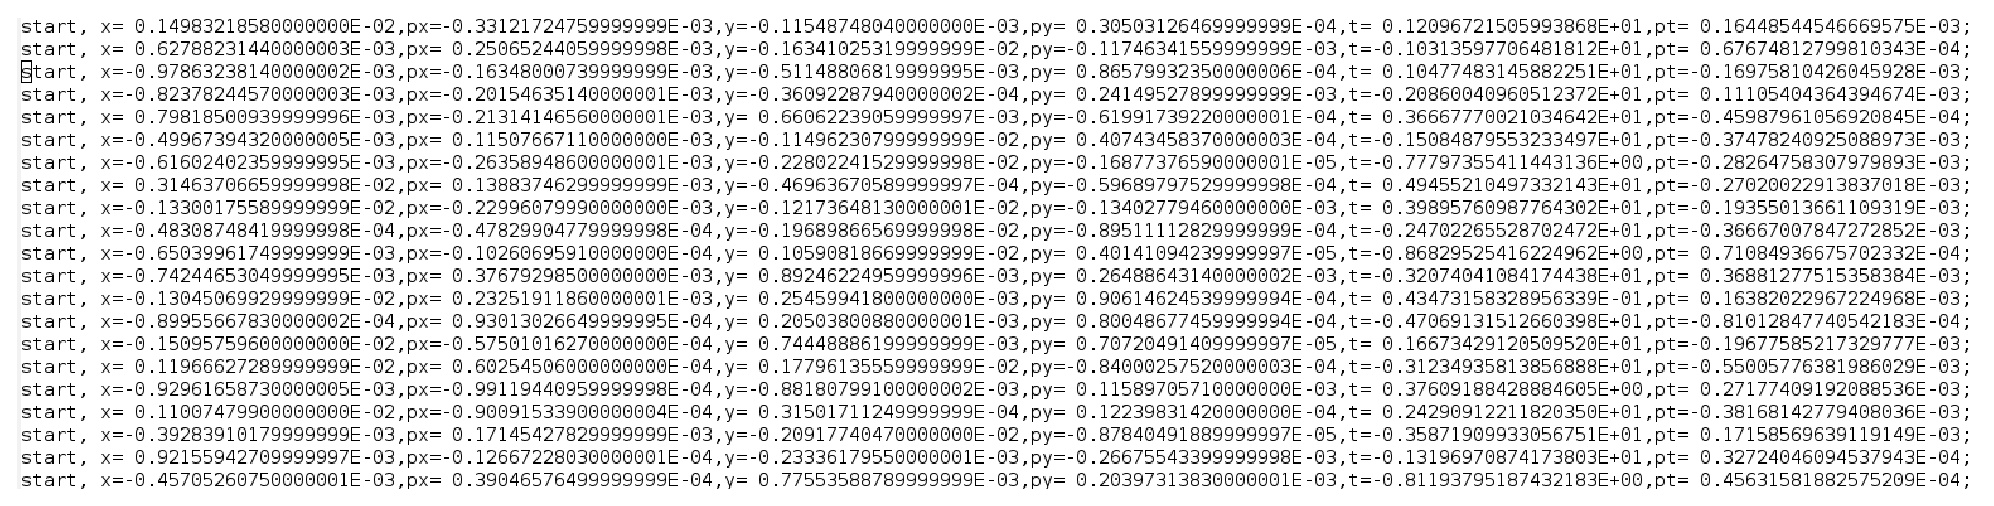
\includegraphics[height=4cm]{eps/start_coordinates}
\caption{Example of a start coordinates file.}
\label{START}
\end{figure}

\subsection{Set-Up Example}\label{SETUP}

In this section it will be described how the user's MAD-X lattice will
be instrumented with thin SC kicks. As an arbitrary example we are
using the CERN PS. It uses MAD-X internal routines and a set MAD-X
control and MACRO files.

This set-up is documented at the web-site:
\href{https://cernbox.cern.ch/index.php/s/olVfNdB8RsfYaCD}{Set-up of MAD-X with Space Charge}

One finds the following directories:
\begin{enumerate}
\item{\bf Manual}\newline
  There, one will find updated versions of this manual.
\item{\bf 6D-Matched-Distribution}\newline
  This MAD-X SC implementation requires 6D linearly matched
  distributions of a couple of 1'000 macro-particles. One finds all
  tools and instructions to prepare such distributions adapted to the
  user's machine case.
\item{\bf Set-Up\_Macros}\newline
  \begin{enumerate}
    At this location one finds the following directories:
  \item{\bf PS-example}\newline
    This directory hold's a fully instantiated example run for the
    CERN PS. It has been run on the CERN lxplus system via the
    command, given that one has placed ``~mad/bin'' in the LINUX
    \$PATH environment:
    \begin{verbatim}
madx make_machine_sequence.madx | tee out_1
  \end{verbatim}
    The MAD-X executables with Space Charge can be downloaded at the
    web at:
%\htmladdnormallink{MAD-X with SC Executables}{http://frs.web.cern.ch/frs/Source/madX_SC/exec}.
%\htmladdnormallink{MAD-X with SC Executables}{https://cern.ch/madx/releases/last-rel/}.

The relevant output file is
    ``ring\_seq\_bb\_spch\_thin.madx''. This is the thin lens PS
    lattice file instrumented with SC kicks at a particular tune
    working point. This file is one of essential input file for
    the SC simulation together with the 6D linearly matched
    distributions, as discussed above.
  \item{\bf Generic-Macros}\newline
    In this directory one finds the generic MACROs that should work
    for any machine case. In Appendix~\ref{APPENDIX2} the input file
    ``madx\_spch\_input.madx'' is explained that allows the standard
    user to modify a title in the Set-Up procedure. More relevant is
    the main input file ``make\_machine\_sequence.madx'' which is
    discussed in Appendix~\ref{APPENDIX3}. Basically, this file
    consist of a part 1 where the user is required to set-up and
    simplify the lattice of the particular machine case to be
    studied. This is followed by part 2 where, after some standard
    MAD-X commands, the user is required to specify the machine
    parameters like ``kinetic\_energy\_gev'' and 2 MACRO control
    parameters explained in the Appendix. Last, for reference of the
    purpose of the applied MACROs in Appendix~\ref{APPENDIX4} the file
    ``main\_make\_spch.madx'' is shown. The standard user will not be
    required to change anything in that file.
  \end{enumerate}
\end{enumerate}

\subsection{Run Example}

In Fig.~\ref{RUN_EXAMPLE} the SC tracking part of a typical runs is
depicted:
\begin{itemize}
\item In a first step the TFS tables {\bf time\_var\_mul} for time
  varying multipoles are read-in (see Fig.~\ref{TIME_VAR_MUL}). The
  first column has the element name, the second is the running number
  of different multipoles. In this case there are 3 different
  sextupoles. The next column gives the number of turns after which
  the multipole strength will be changed. If turn numbers are missing
  no change of the multipoles will be applied for those turn
  numbers. The following 20 columns are reserved for multipoles of up
  to $10^{th}$ order. The normal coefficients are followed by the skew
  ones: i.e. normal dipole, vertical dipole, normal quadrupole, skew
  quadrupole, normal sextupole etc. In this example the normal
  sextupoles (fifth multipole column) hold values different from
  zero. The remaining 15 columns are not shown.

  Then the TFS table of phase trombone {\bf time\_var\_pha} is read-in
  (see Fig.~\ref{TIME_VAR_PHA}). It has the same structure as the TFS
  table for multipoles. However, in this case the 36 matrix elements
  are contained in this table (32 columns have been suppressed in the
  figure). In this example there is only one phase trombone.

  This example contains no time varying cavity. The {\bf
    time\_var\_cav} file would just have the necessary first 3 columns
  and a single column with the desired {\bf VOLT} in [MV].
\item Notice that after any TWISS command one has to read-in the table
  {\bf  spch\_bb\_twiss\_ini.dat}.
\item A set of flags are needed to activate the SC treatment.
\item The MAD-X {\bf TRACK} environment is being opened and the start
  coordinates are being read-in.
\item On the MAD-X {\bf RUN} command special care has been taken to
  avoid numerical exception by defining the RF bucket.
\item A run with a single turn is followed by a loop of runs with a
  TWISS parameter recalculation after every turn at all positions of
  the SC elements. Notice, that the table {\bf
    spch\_bb\_twiss\_ini.dat} has to be read-in after each TWISS command.
\item Last, the tracking output is written out for the emittance
  evolution, the final TWISS parameters, the 6D coordinate printout
  and the record of lost particles respectively.
\item Fig.~\ref{RUN_EXAMPLE_3D} shows a {\bf RUN EXAMPLE} available
  in the implementation after 2018 featuring the flags {\bf
    sc\_3d\_kick}, {\bf sc\_3d\_periodic=TRUE} (``periodic'' mode) and
    {\bf sc\_3d\_periodic=false} (``free'' mode), see above for more
    details.

\end{itemize}

%\newpage
\begin{figure}[H]
\centering 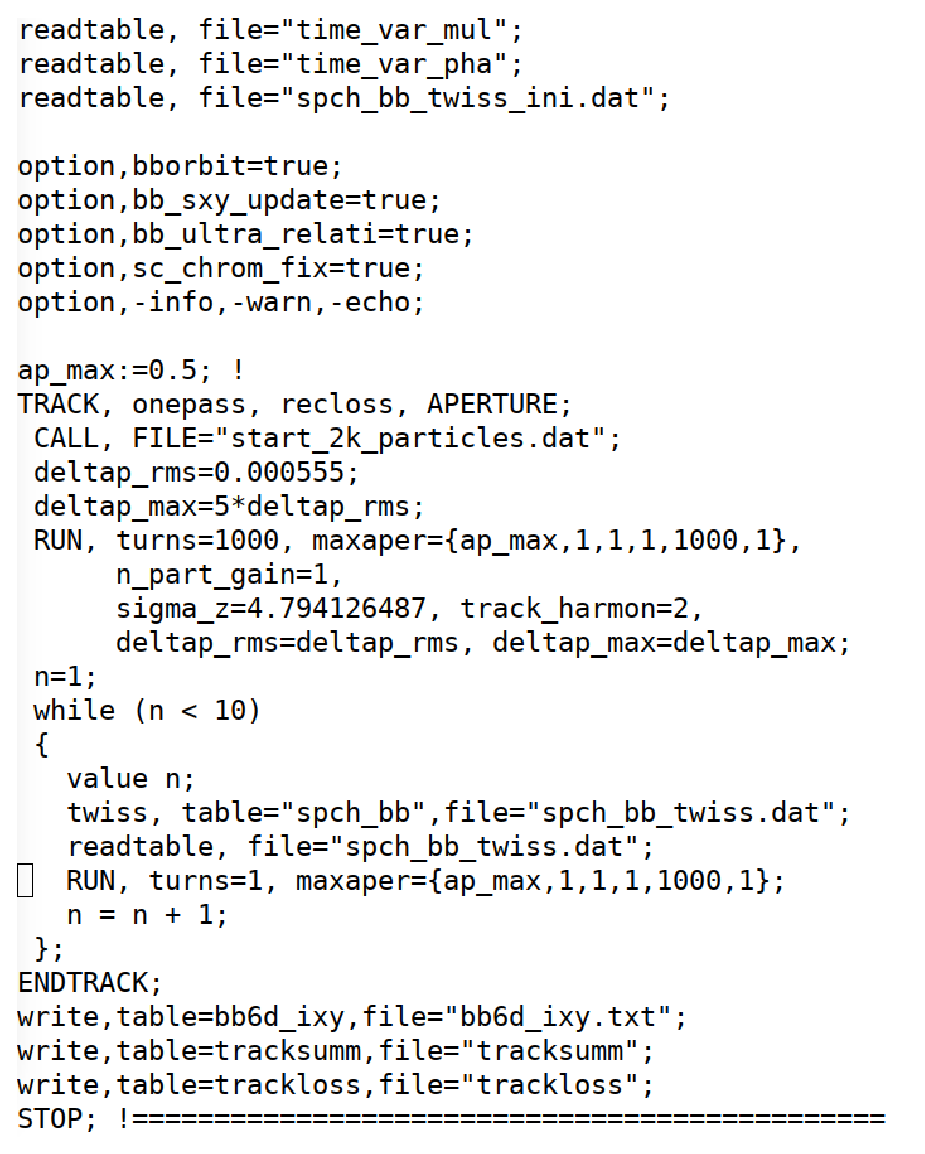
\includegraphics[width=8cm]{eps/run_example2_new}
\caption{A typical run example before the 2018 implementation,
  i.e. adaptive and purely frozen mode.}
\label{RUN_EXAMPLE}
\end{figure}

\newpage
\begin{figure}[H]
\centering 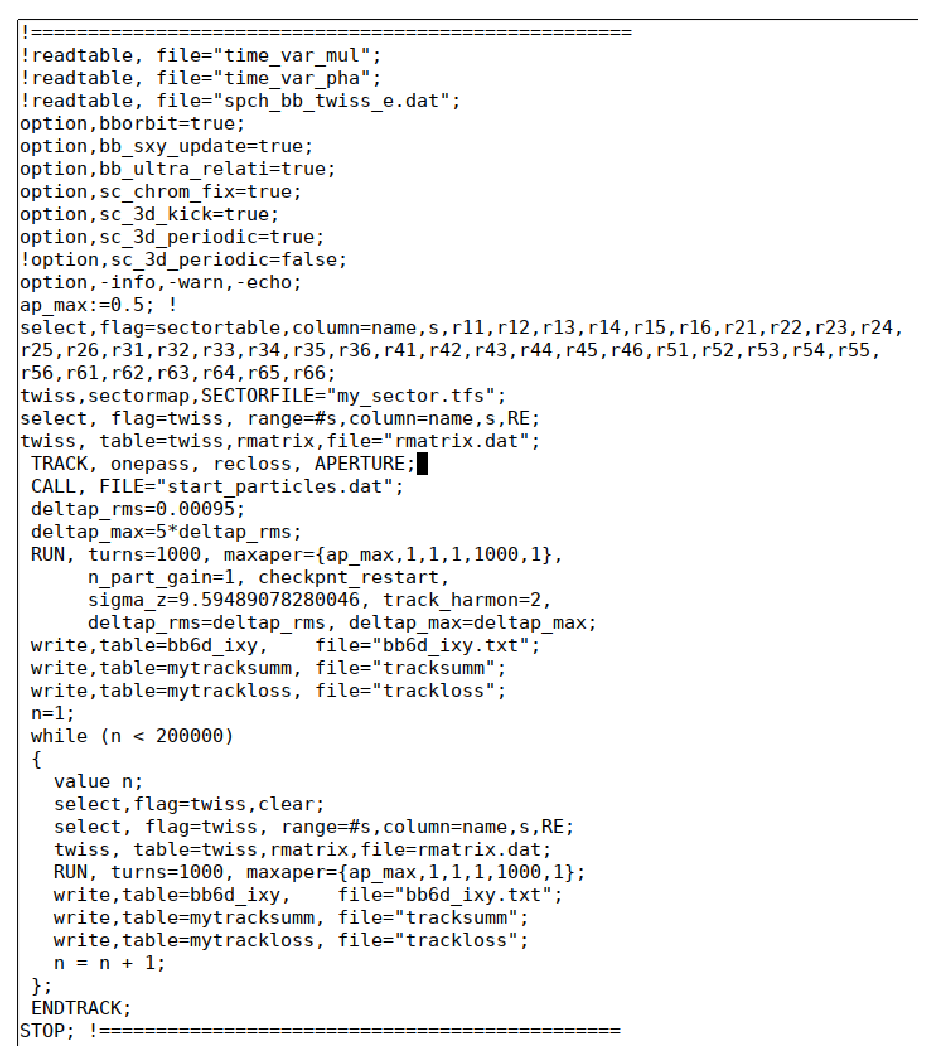
\includegraphics{eps/run_example_3D2_new}
\caption{A typical run example after 2018 implementation,
  i.e. with the symplectic SC 3D kick and ``periodic'' or
  ``free''(self-consistent) mode.}
\label{RUN_EXAMPLE_3D}
\end{figure}

\newpage
\begin{figure}[H]
\centering
\begin{minipage}[b]{0.45\linewidth}
  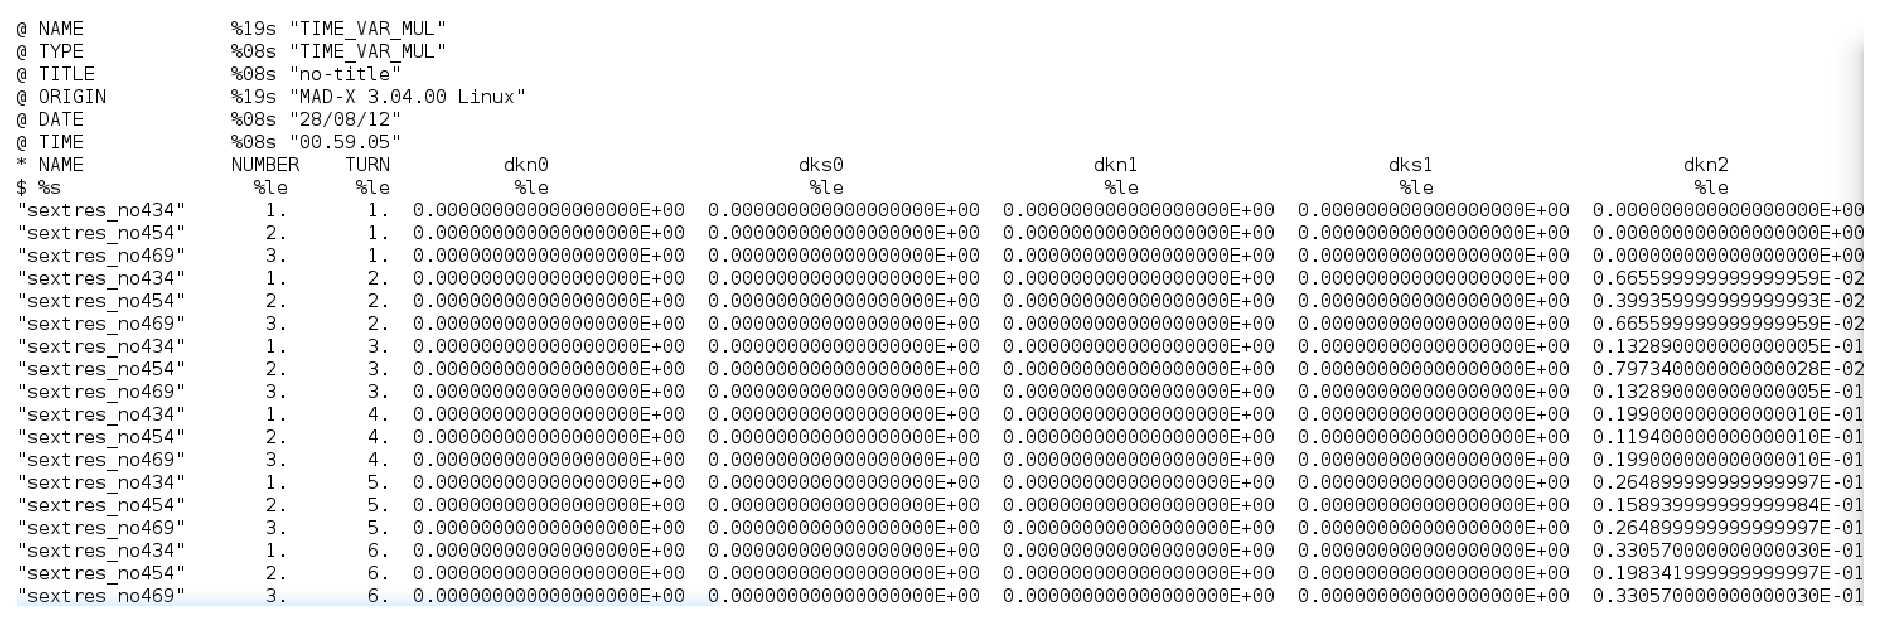
\includegraphics[height=7cm,angle=-90]{eps/cut_out_time_var_mul}
\caption{Example of a Time Variation Multipole TFS table.}
\label{TIME_VAR_MUL}
\end{minipage}
\quad
\begin{minipage}[b]{0.45\linewidth}
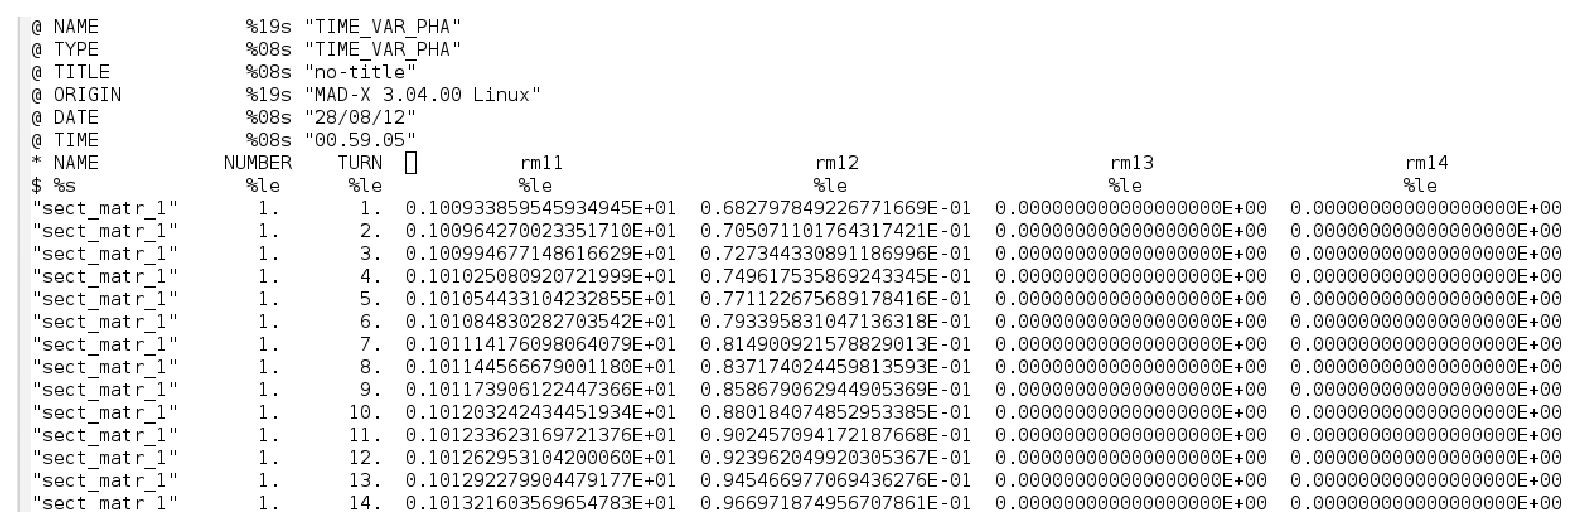
\includegraphics[height=7cm,angle=-90]{eps/cut_out_time_var_pha}
\caption{Example of a Time Variation Phase Trombone TFS table.}
\label{TIME_VAR_PHA}
\end{minipage}
\end{figure}

\subsection{Laslett Tune Shift Formulae}\label{SEC:LASLETT}

Here the formula as used in the file {\bf
  spcharge\_laslett\_tune\_shift.madx} in the third step of the
preparatory phase-I, with the tunes from TWISS:
\begin{equation}
\nu_{x, y},
\end{equation}
averaged $\bar{\beta}$ value and length of the machine
$L_{\textrm{ring}}$ relate:
\begin{equation}
\bar{\beta}_{x, y} = \frac{L_{\textrm{ring}}}{2\pi\nu_{x, y}},
\end{equation}
and averaged $\bar{\sigma}$:
\begin{equation}
\bar{\sigma}_{x, y} = \sqrt{\epsilon_{x, y}\bar{\beta}_{x, y}},
\end{equation}
the SC tune-shift reads:
\begin{equation}\label{LASLETT}
\Delta\nu_{x, y} = \frac{r_pN_p \cdot \bar{\beta}_{x, y}}{2\pi\cdot
  B_f \cdot \gamma^3 \beta^2 \cdot \bar{\sigma}_{x, y}(\bar{\sigma}_x
  + \bar{\sigma}_y)},
\end{equation}
with $B_f$ as the bunching factor.\\ \mbox{ }\\ For the particular
case of bunched Gaussian beams the SC tune shift formula reads as
follows:
\begin{equation}\label{LASLETT-BUNCH}
\Delta\nu_{x, y} = \frac{r_pN_p}{(2\pi)^{\frac{3}{2}} \cdot \gamma^3
  \beta^2 \cdot \sigma_z}\cdot \oint{\frac{\beta_{x, y}(s) \cdot
    ds}{\sigma_{x, y}(s)(\sigma_x(s) + \sigma_y(s))}}.
\end{equation}
After integration one gets:
\begin{equation}
\Delta\nu_{x, y} = \frac{r_pN_p \cdot \bar{\beta}_{x,
    y}}{(2\pi)^{\frac{3}{2}} \cdot \gamma^3 \beta^2 \cdot
  \frac{\sigma_z}{L_{\textrm{ring}}} \cdot \bar{\sigma}_{x,
    y}(\bar{\sigma}_x + \bar{\sigma}_y)}.
\end{equation}
The bunching factor can be defined as the ratio of the ``effective
length'' $L^{\textrm{eff}}_{\textrm{bunch}}$ to the length of the ring
$L_{\textrm{ring}}$.
\begin{equation}
B_f = \frac{L^{\textrm{eff}}_{\textrm{bunch}}}{L_{\textrm{ring}}}.
\end{equation}
where the "effective" bunch length can be seen as the length of an
ideal bunch with uniform distribution, which contains the same number
of particles as a bunch with an arbitrary non-uniform distribution,
e.g. a Gaussian bunch.

This implies that for Gaussian beams with the
$L^{\textrm{eff}}_{\textrm{bunch}} = \sqrt{2\pi} \cdot \sigma_z$ the
bunching factor $B_f$ should read:
\begin{equation}\label{BF}
B_f = \sqrt{2\pi} \cdot \frac{\sigma_z}{L_{\textrm{ring}}}.
\end{equation}

\subsection{Beam Modes}
Remarks on the transition from coasting to non-monochromatic and then
to bunched beams.

Demonstrated with a numerical example for the FNAL
debuncher~\cite{KAPIN-I}:
\begin{itemize}
\item[1.)]  For {\bf coasting} 4D beam $N=1.75\cdot10^{13}$ with a
  tune shift of $\Delta\nu=-0.0148$ there is a good agreement between
  the analytic Laslett's tune shift (at $B_f=1$) and the numerical
  TWISS determination.

\item[2.)]  For non-monochromatic beams in the debuncher, let's take
  into account the well-known Formulae for the beam size in the arcs
  with ($D>0$) for bunches with significant momentum
  spread~\cite{MACKEY}:
  \begin{equation}\label{DISP}
    \sigma^2_{tot}= \sigma^2_\beta + [D_x(s) \sigma_p]^2.
  \end{equation}
  With ($\sigma_p=4.5\cdot10{-3}$) and due to the large $D_x$ the tune
  shift reduces to ($\Delta\nu=-0.0054$). This value has been
  calculated numerically via MAD-X with both TWISS commands using Eq.~\ref{DISP}
  and TBT tracking over 1024 turns. Therefore, one should increase
  Npart for SC-elements by a factor of $N\_part\_gain=2.7$, i.e. by
  $\frac{0.0148}{0.0054}$, to get back ($\Delta\nu=-0.0148$) as for
  non-monochromatic beams.
\item[3.)] Number of particles in coasting and bunched beam producing
  the same Laslett tune shift:
  \begin{equation}
    \begin{split}
      Npart(6D)= Npart(4D, B_f=1) * N\_part\_gain * B_f=\\ Npart(4D,
      B_f=1) * N\_part\_gain *
      (\sqrt{2\pi}*\sigma_z/L_{\textrm{ring}})=\\
1.75\cdot10^{13}*(2.7)*(2.5*12/505)=2.8\cdot10^{12}.
  \end{split}
  \end{equation}
\end{itemize}
\subsubsection{General MAD-X Set-Up Input}\label{APPENDIX2}
The user may modify the input file ``madx\_spch\_input.madx''. In
particular the {\it\bf title\_madx\_script} entry maybe modified to
the user's taste: it will appear in MAD-X output files during the
Set-Up phase and does not alter the outcome otherwise. Changing the
other two items is discouraged and should only be performed by experts
since it will require various other changes in the generic MACROS.
\begin{verbatim}
*****************************************************************************
input file: madx_spch_input.madx:
********************************
&input_filename
twiss_element_list_filename='twiss_element_list.txt'
                 ! created in 1a_step
&END

&madx_job_title
title_madx_script='2021: PS Run'
&END

&ring_seq_filename
filename_ring_elements_seq='machine_sequence.madx'
                       ! ring sequence with SAVE, SEQUENCE=<>,file=<>.madx;
&END
*****************************************************************************
\end{verbatim}

\subsubsection{Preparing MAD-X Lattice for SC Kicks}\label{APPENDIX3}
The main input file ``make\_machine\_sequence.madx'' consist of a
user defined simplified original lattice definition of the user's
machine case. This part is followed by some generic MAD-X commands
and a list of input parameters that the user needs to adapt to his case.
This second part of the file is depicted below. Besides evident
parameters like ``kinetic\_energy\_gev'' there are 2 relevant
parameters:
\begin{enumerate}
\item{\bf L\_div\_max}\newline
  This parameter defines the maximum distance between 2 SC kicks in
  [m]. For the PS we have been using 1 [m] which has allowed for a
  dense enough coverage of SC kicks around the machine and about 1'100
  kicks seems good enough. Obviously, one should not overdo the number
  of kicks because this number is directly proportional to the
  execution time of the run. As an example: for the PS 500'000 turns
  take about 6 weeks computing time on modern computer PCs.
\item{\bf delta\_nu\_min}\newline
  The MAD-X SC Set-Up procedure is turning on the strength of the SC
  kicks adiabatically to avoid potential TWISS command crashes because the
  strength of the SC kicks depend on the TWISS parameters itself. The
  {\it\bf delta\_nu\_min} parameter controls the speed of the
  convergence. Typically we are using {\it\bf delta\_nu\_min=0.25} but
  for the PS we needed to do it in finer steps: {\it\bf
    delta\_nu\_min=0.07}.
\end{enumerate}
\begin{verbatim}
*****************************************************************************
input part of file: make_machine_sequence.madx:
***********************************************
!
! Create file=twiss_element_list.txt printing element list
 SELECT, flag=twiss,clear;
 SELECT, flag=twiss, column=name, keyword, L;
 TWISS, file=twiss_element_list.txt;

! Do former "2_step MAD-X SC internally
 option,sc_setup=true; ! required do not change
 TWISS;
 option,sc_setup=false; ! required do not change

! Write out the machine sequence as file=machine_sequence.madx
 SAVE,SEQUENCE=MACHINE,file=machine_sequence.madx;
 call,file=machine_sequence.madx;

!
!Machine Parameters: Example PS
!
!Parameters to be set
kinetic_energy_gev =   2.0 ;
Ex_norm=3.5E-6 ; ! Normalized horizontal emittance
Ey_norm=2.2E-6 ; ! Normalized vertical emittance
Bunch_length_4s=135e-9 ; ! 4 sigma bunch_length [ns]
NPART_tot=55e10 ; ! Total number of particles in the machine
L_div_max=1.; value, L_div_max;  ! Upper limit for segment length
delta_nu_min=0.07; ! Typical 0.25; ! FRS 02.09.2020 Constant for tune-shift of PS

L_ring:=table(summ,length);
value, L_ring;
rest_energy_gev =   pmass ;
total_energy_GeV:=kinetic_energy_GeV+rest_energy_GeV;
gamma=total_energy_GeV/rest_energy_gev;
beta=sqrt(1.-1./gamma^2);
value, gamma,beta;
Ex_spch:=Ex_norm/gamma/beta; Ey_spch:=Ey_norm/gamma/beta; ! [m] ! PS tracking
Bunch_length:= Bunch_length_4s/4.*clight*beta; ! PS 1 RMS bunchlength in [m]
value,Bunch_length, clight, beta;
NPART:=NPART_tot*L_ring/Bunch_length/sqrt(2*pi); ! PS new definition
value, NPART;
N_spch:=SC_count-1;
value, L_div_max,N_spch,SC_count,delta_nu_min;

! EXPERTS Usuage only! Needed for backwards compatibility mode
CALL, FILE=input_compatibility.madx; ! required do not change

! Do former "3_step" with generic MACROs
CALL, FILE=main_make_spch.madx; ! required do not change
stop;
*****************************************************************************
\end{verbatim}

\subsubsection{Adiabatic Switching on SC}\label{APPENDIX4}
The execution of the MACROs is controlled by the file
``main\_make\_spch.madx''. There is no need to modify this file by
the standard user. It is just shown for a reference of the purpose of
each individual MACRO.
\begin{verbatim}
*****************************************************************************
input file: main_make_spch.madx:
*******************************
! Start file: "main_make_spch.madx"
! Calling MACROS
option,info,warn,echo,bb_ultra_relati;
set,format="24.16e";
debug_print=0;

value,rest_energy_GeV,kinetic_energy_GeV,total_energy_GeV,clight,gamma,
beta,Bunch_length,N_particles,Z_particle,A_particle,r0_particle,prad,L_div_max;

CALL FILE=spcharge_macro_20090316.madx;

! backwards compatibility mode
!CALL FILE=spcharge_constants_and_formulae.madx; ! <= constants for space charge

! backwards compatibility mode
!CALL FILE=spcharge_input_parameters.madx; ! <=input parameters for space charge

Call FILE=spcharge_beam_command.madx;     ! BEAM command

CALL FILE=spcharge_ring_seq.madx;       ! <= read lattice sequence
                                        ! with universal name (file generated by CVF)

USE, PERIOD=ring; TWISS;

Call FILE=spcharge_beam_command.madx;     ! second BEAM command

! =====  Analytical  tune shift ===============================
CALL FILE=spcharge_laslett_tune_shift.madx; ! <= Analytical evaluation 

debug_print=0;

CALL FILE=spcharge_matrix.madx;

debug_print=0;

CALL FILE=spcharge_bbkick.madx;

! MAKETHIN
CALL, FILE = spcharge_makethin.madx;

twiss;
emit;
stop;
! End file: "main_make_spch.madx"
! End MAD-X file "make_machine_sequence.madx"
\end{verbatim}
*****************************************************************************

%% EOF
